\documentclass[
11pt, % The default document font size, options: 10pt, 11pt, 12pt
%codirector, % Uncomment to add a codirector to the title page
]{charter} 


% El títulos de la memoria, se usa en la carátula y se puede usar el cualquier lugar del documento con el comando \ttitle
\titulo{Interfaces Cerebro-Cloud para la predicción de actividades de imaginación motriz}

% Nombre del posgrado, se usa en la carátula y se puede usar el cualquier lugar del documento con el comando \degreename
%\posgrado{Carrera de Especialización en Sistemas Embebidos} 
%\posgrado{Carrera de Especialización en Internet de las Cosas} 
\posgrado{Carrera de Especialización en Inteligencia Artificial}
%\posgrado{Maestría en Sistemas Embebidos} 
%\posgrado{Maestría en Internet de las cosas}

% Tu nombre, se puede usar el cualquier lugar del documento con el comando \authorname
% IMPORTANTE: no omitir titulaciones ni tildación en los nombres, también se recomienda escribir los nombres completos (tal cual los tienen en su documento)
\autor{Ing. Freddy Julian Riascos Salas}

% El nombre del director y co-director, se puede usar el cualquier lugar del documento con el comando \supname y \cosupname y \pertesupname y \pertecosupname
\director{Mg. Ing. Jaime Andrés Riascos Salas}
\pertenenciaDirector{Potsdam Embodied Cognition Group PECoG} 
\codirector{} % para que aparezca en la portada se debe descomentar la opción codirector en los parámetros de documentclass
\pertenenciaCoDirector{FIUBA}

% Nombre del cliente, quien va a aprobar los resultados del proyecto, se puede usar con el comando \clientename y \empclientename
\cliente{Xprende}
\empresaCliente{Xprendetech S.A}
 
\fechaINICIO{4 de marzo de 2025}		%Fecha de inicio de la cursada de GdP \fechaInicioName
\fechaFINALPlan{22 de abril de 2025} 	%Fecha de final de cursada de GdP
\fechaFINALTrabajo{octubre de 2025}	%Fecha de defensa pública del trabajo final


\begin{document}

\maketitle
\thispagestyle{empty}
\pagebreak


\thispagestyle{empty}
{\setlength{\parskip}{0pt}
\tableofcontents{}
}
\pagebreak


\section*{Registros de cambios}
\label{sec:registro}


\begin{table}[ht]
\label{tab:registro}
\centering
\begin{tabularx}{\linewidth}{@{}|c|X|c|@{}}
\hline
\rowcolor[HTML]{C0C0C0} 
Revisión & \multicolumn{1}{c|}{\cellcolor[HTML]{C0C0C0}Detalles de los cambios realizados} & Fecha      \\ \hline
0      & Creación del documento                                 &\fechaInicioName \\ \hline
1      & Se completa hasta el 5 punto inclulsive                & 20 de marzo de 2025 \\ \hline
2      & Se completa hasta el 8 punto inclulsive               & 28 de marzo de 2025 \\ \hline
%1      & Se completa hasta el punto 5 inclusive                & {día} de {mes} de 202X \\ \hline
%2      & Se completa hasta el punto 9 inclusive
%		  Se puede agregar algo más \newline
%		  En distintas líneas \newline
%		  Así                                                    & {día} de {mes} de 202X \\ \hline
%3      & Se completa hasta el punto 12 inclusive                & {día} de {mes} de 202X \\ \hline
%4      & Se completa el plan	                                 & {día} de {mes} de 202X \\ \hline

% Si hay más correcciones pasada la versión 4 también se deben especificar acá

\end{tabularx}
\end{table}

\pagebreak



\section*{Acta de constitución del proyecto}
\label{sec:acta}

\begin{flushright}
Buenos Aires, \fechaInicioName
\end{flushright}

\vspace{2cm}

Por medio de la presente se acuerda con el \authorname\hspace{1px} que su Trabajo Final de la \degreename\hspace{1px} se titulará ``\ttitle'' y consistirá en \textit{evaluar una interfaz cerebro-computadora (Brain-Computer Interface}, BCI) \textit{con soporte en la nube para la detección de patrones de imaginación motriz}. El trabajo tendrá un presupuesto preliminar estimado de 600 horas y un costo estimado de \$25000, con fecha de inicio el \fechaInicioName\hspace{1px} y fecha de presentación pública en \fechaFinalName.

Se adjunta a esta acta la planificación inicial.

\vfill

% Esta parte se construye sola con la información que hayan cargado en el preámbulo del documento y no debe modificarla
\begin{table}[ht]
\centering
\begin{tabular}{ccc}
\begin{tabular}[c]{@{}c@{}}Dr. Ing. Ariel Lutenberg \\ Director posgrado FIUBA\end{tabular} & \hspace{2cm} & \begin{tabular}[c]{@{}c@{}}\clientename \\ \empclientename \end{tabular} \vspace{2.5cm} \\ 
\multicolumn{3}{c}{\begin{tabular}[c]{@{}c@{}} \supname \\ Director del Trabajo Final\end{tabular}} \vspace{2.5cm} \\
\end{tabular}
\end{table}




\section{1. Descripción técnica-conceptual del proyecto a realizar}
\label{sec:descripcion}

% ELIMINAR \begin{consigna}{red} y \end{consigna}{red} en las secciones que vayan completando para cada entrega parcial.
Las interfaces cerebro-computadora (\textit{Brain-Computer Interfaces}, BCI) han emergido como una tecnología innovadora que permite la comunicación directa entre el cerebro humano y dispositivos externos.
En particular, la predicción de actividades de imaginación motriz a través de BCI han cobrado relevancia en campos que varían desde la rehabilitación, robótica, control de protésis hasta sistemas domóticos, videojuegos y realidad virtual.

La integración de las BCI con tecnologías en la nube permite el almacenamiento, procesamiento y análisis eficiente de grandes volúmenes de datos cerebrales. Esto favorece la aplicación de algoritmos avanzados de aprendizaje automático y mejora la precisión de la interpretación de señales cerebrales.

\textbf{1.1 Conceptos fundamentales}

Interfaces cerebro-computadora

Los BCI son sistemas que registran la actividad cerebral mediante técnicas como la electroencefalografía (EEG) y traducen estas señales en comandos computacionales. Existen distintos tipos de BCI:
\begin{itemize}
	\item Invasivas: electrodos implantados directamente en el cerebro.
	\item No invasivas: uso de sensores externos como EEG, MEG o fNIRS.
\end{itemize}

Imaginación motriz

La imaginación motriz se refiere a la capacidad de representar mentalmente movimientos sin ejecutarlos físicamente. Durante este proceso, se activan patrones específicos en la corteza motora, los cuales pueden ser detectados mediante EEG y utilizados para el control de dispositivos externos.

Computación en la nube y BCI

El uso de servicios en la nube permite procesar grandes volúmenes de datos EEG en tiempo real obteniendo beneficios como:
\begin{itemize}
	\item Almacenamiento y procesamiento escalable de datos cerebrales.
	\item Acceso remoto para análisis colaborativo.
	\item Implementación de modelos de aprendizaje automático en infraestructura distribuida.
\end{itemize}

\textbf{1.2 Problema actual}

Al presente, las personas con discapacidades motoras severas enfrentan grandes dificultades en la interacción con su entorno. Los sistemas actuales de BCI presentan limitaciones en términos de precisión, latencia, accesibilidad, recopilación,
análisis y clasificación de las señales EEG. Normalmente, estos datos se encuentran contaminados por distintos artefactos biológicos, tales como señales cardíacas, respiratorias o músculos, como también por ruidos externos.

Así mismo, la dimensión de estos datos, dada por la cantidad de canales y señal de tiempo, crea una problema de procesamiento y dimensionalidad. Todas estas dificultades evitan que el clasificador reciba características latentes de la señal y así realizar la predicción de forma adecuada y rápida.

\textbf{1.3 Solución propuesta}

La interfaz Cerebro-Cloud sugerida integra un modelo de predicción basado en aprendizaje automático con una arquitectura en la nube que permita la adquisición, procesamiento y transmisión de señales cerebrales en tiempo real. Esto proporcionará una solución más precisa, escalable y accesible para el control
de dispositivos mediante imaginación motriz.



En comparación con el estado del arte actual, la solución se destaca en:

\begin{itemize}
	\item Precisión mejorada: uso de modelos de inteligencia artificial optimizados para la interpretación de señales eléctricas (electroencefalografía, EEG).
	\item Reducción de latencia: procesamiento distribuido en la nube.
	\item Accesibilidad: plataforma escalable con acceso a la información para usuarios y especialistas.
\end{itemize}

Este interfaz BCI-Cloud tiene como objetivo mejorar la calidad de vida de personas con discapacidades motoras
al proporcionar una herramienta en la nube para la comunicación y control de dispositivos protésicos.

El proyecto se enmarca dentro de un programa de innovación tecnológica de la empresa \clientename, que cuenta con financiamiento para su ejecución.

\textbf{1.4 Descripción funcional y diagrama en bloques}

La solución propuesta consta de los siguientes módulos principales:
\begin{itemize}
	\item Adquisición de señales EEG: sensores no invasivos capturan la actividad cerebral del usuario.
	\item Preprocesamiento de datos: filtrado y eliminación de ruido en las señales EEG.
	\item Modelo de predicción: algoritmos de aprendizaje automático analizan los datos y determinan la intención motriz.
	\item Transmisión en la nube: los datos procesados se envían a servidores remotos para análisis y almacenamiento.
	\item Interfaz usuario-dispositivo: una interfaz que traduce la predicción en comandos para dispositivos externos, como prótesis o interfaces de control.
\end{itemize}

En la figura 1 se presenta el diagrama de bloques del sistema BCI-Cloud. Se observa que el usuario inicial genera datos con el sensor EEG. Luego envía los datos a un sistema de preprocesamiento. 
Una vez que los datos se encuentran óptimos se envian a la nube. Seguidamente el modelo seleccionado se entrena. Finalmente el modelo predice el movimiento imaginado en la interfaz de usaurio.

\begin{figure}[htpb]
\centering 
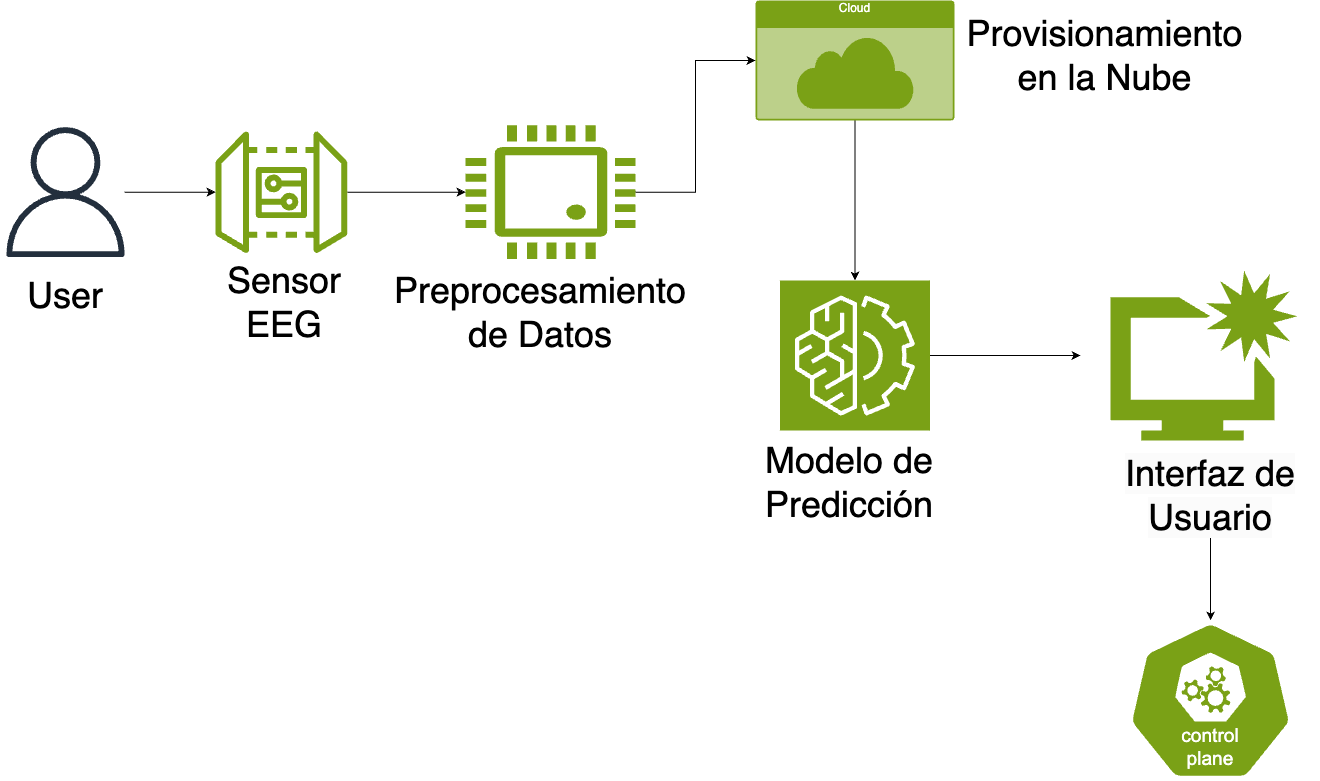
\includegraphics[width=.65\textwidth]{./Figuras/block_diagram.png}
\caption{Diagrama del sistema BCI-Cloud.}
\label{fig:diagBloques}
\end{figure}

\vspace{25px}

% ELIMINAR \begin{consigna}{red} y \end{consigna}{red} en las secciones que vayan completando para cada entrega parcial.

\section{2. Identificación y análisis de los interesados}
\label{sec:interesados}

A continuación, se presentan los principales actores involucrados en el desarollo del proyecto y su respectiva función:
 
\begin{table}[ht]
%\caption{Identificación de los interesados}
%\label{tab:interesados}
\begin{tabularx}{\linewidth}{@{}|l|X|X|l|@{}}
\hline
\rowcolor[HTML]{C0C0C0} 
Rol           & Nombre y Apellido & Organización 	& Puesto 	\\ \hline
Cliente       & Ing. Miguel Amaya       &\empclientename	& -       	\\ \hline
Responsable   & \authorname       & FIUBA        	& Alumno 	\\ \hline
Orientador    & \supname	      & \pertesupname 	& Director del Trabajo Final \\ \hline
Usuario final & Paciente          & -             	& -        	\\ \hline
\end{tabularx}
\end{table}

A continuación las principales características de cada interesado.
 
\begin{itemize}
	\item Orientador: el Mg. Ing. Andrés Salas es experto en desarrollar interfaces cerebro-maquina y dará orientación con la definición de los requerimientos y el desarrollo del sistema BCI-Cloud.
	\item Usuario final: usuario con discapacidad motora severa, quien se beneficiaría directamente del control del dispositivo y la interfaz.
\end{itemize}

% ELIMINAR \begin{consigna}{red} y \end{consigna}{red} en las secciones que vayan completando para cada entrega parcial.
\section{3. Propósito del proyecto}
\label{sec:proposito}
La intención del proyecto es diseñar y desarrollar una plataforma basada en BCI-Cloud que facilite la predicción de actividades de imaginación motriz en personas con discapacidades motoras severas. A través de la integración de inteligencia artificial y computación en la nube, se busca ofrecer una solución innovadora que permita mejorar la interacción con el entorno mediante el control preciso de dispositivos electrónicos y protésicos.

\section{4. Alcance del proyecto}
\label{sec:alcance}

El proyecto comprenderá los siguientes componentes:
\begin{itemize}
	\item Modelo de predicción basado en algoritmos de aprendizaje automático para la interpretación de señales EEG. Se evaluarán distintos modelos como CNNs, RNNs y \textit{Transformers} para determinar el que mejor performe en términos de precisión y latencia.
	\item Datos adquiridos de sensores EEG, que se utilizarán para entrenar y validar el modelo. Se garantizará que la adquisición de datos cumpla con estándares de calidad y se preprocesen para eliminar ruido.
	\item Código de la infraestructura en la nube.
	\item Documentación técnica y científica, que detalla el diseño, implementación y validación del sistema.
	\item Pruebas y validaciones realizadas con usuarios objetivo para evaluar el desempeño y precisión del modelo. Se incluirán métricas clave que garanticen el óptimo desempeño del sistema.
	\item Desarrollo y entrenamiento del modelo de predicción de actividades de imaginación motriz, con comparaciones entre distintos enfoques de inteligencia artificial.
	\item Integración con una infraestructura en la nube escalable y segura en \textit{Amazon Web Services}.
	\item Adquisición y procesamiento de señales cerebrales mediante sensores EEG.
	\item Evaluación del sistema con usuarios finales para validar su precisión y usabilidad.
	\item Generación de documentSación técnica para futuras mejoras e implementación.
	\item Optimización del procesamiento en la nube para reducir latencia y mejorar la eficiencia del sistema.
\end{itemize}
El presente proyecto no incluye:
\begin{itemize}
	\item Desarrollo de hardware EEG propio. Para ello se utilizarán dispositivos comerciales disponibles en el mercado.
	\item Implementación de interfaces cerebro-máquina más allá de la imaginación motriz.
	\item Integración con sistemas de salud o bases de datos clínicas.
\end{itemize}

% ELIMINAR \begin{consigna}{red} y \end{consigna}{red} en las secciones que vayan completando para cada entrega parcial.


\section{5. Supuestos del proyecto}
\label{sec:supuestos}
\begin{itemize}
	\item Disponibilidad de datos EEG de calidad: se asume que los datos recopilados mediante sensores EEG serán suficientes y de calidad adecuada para el entrenamiento del modelo sin necesidad de un preprocesamiento excesivo.
	\item Recursos computacionales: se cuenta con acceso a instancias de cómputo en la nube, tales como las brindadas por \textit{Amazon Web Services}, que permitan el entrenamiento y despliegue del modelo de inteligencia artificial sin limitaciones de procesamiento o almacenamiento.
	\item Factibilidad técnica de integración: se considera viable la integración entre los sensores EEG, la infraestructura en la nube y la interfaz de usuario.
	\item Condiciones regulatorias favorables: no existen restricciones legales o normativas que impidan la recopilación y procesamiento de datos EEG.
\end{itemize}

% ELIMINAR \begin{consigna}{red} y \end{consigna}{red} en las secciones que vayan completando para cada entrega parcial.

\section{6. Product backlog}
\label{sec:backlog}
\begin{enumerate}
	\item Épica 1  Adquisición y procesamiento de datasets EEG
	\begin{enumerate}
		\item HU1 
		
		Como ingeniero, quiero obtener señales EEG desde datasets públicos para alimentar el modelo de predicción.\newline
		
		
		Dificultad: 5
		
		Complejidad: 4 
		
		Incertidumbre: 3
		
		Suma: 12 → \textit{Story Points}: 13
		
		Prioridad: 1\newline
		
		
		\item HU2
		
		Como ingeniero, quiero que las señales EEG sean filtradas y normalizadas automáticamente para mejorar la calidad del entrenamiento del modelo.\newline

		Dificultad: 4 
		
		Complejidad: 2 
		
		Incertidumbre: 2 
		
		Suma: 8 → \textit{Story Points}: 8

		Prioridad: 2\newline

		
	\end{enumerate}
	\item Épica 2  Inteligencia artificial y modelado
	\begin{enumerate}
		\item HU3
		
		Como ingeniero, quiero entrenar un modelo de inteligencia artificial con señales EEG preprocesadas para predecir actividades de imaginación motriz con alta precisión.\newline
		
		Dificultad: 5
		
		Complejidad: 5
		
		Incertidumbre: 4
		
		Suma: 14 → \textit{Story Points}: 21
		
		Prioridad: 3\newline
		
		\item HU4
		
		Como ingeniero, quiero optimizar el modelo de inteligencia artificial para que su inferencia sea menor a 5000 ms, alcance al menos un 80\% de precisión y exponga sus predicciones mediante una API REST.\newline
		
		Dificultad: 4
		
		Complejidad: 3
		
		Incertidumbre: 3
		
		Suma: 10 → \textit{Story Points}: 13

		Prioridad: 4\newline
	\end{enumerate}
	\item Épica 3  Infraestructura en la nube
	\begin{enumerate}
		\item HU5
		
		Como ingeniero, quiero que el procesamiento de datos EEG ocurra en \textit{Amazon Web Services} AWS Lambda para mejorar la escalabilidad del sistema.\newline
		
		Dificultad: 5
		
		Complejidad: 4
		
		Incertidumbre: 3
		
		Suma: 12 → \textit{Story Points}: 13

		Prioridad: 5\newline
		
		\item HU6
		
		Como ingeniero, quiero desplegar automáticamente el modelo entrenado en AWS para facilitar su mantenimiento, escalabilidad y monitoreo.\newline
		
		Dificultad: 4
		
		Complejidad: 3
		
		Incertidumbre: 3
		
		Suma: 10 → \textit{Story Points}: 13

		Prioridad: 6\newline
	\end{enumerate}
	\item Épica 4  Interfaz de usuario y seguridad
	\begin{enumerate}
		\item HU7
		
		Como usuario final, quiero visualizar mis señales EEG en una interfaz gráfica para entender cómo se interpretan mis actividades cerebrales.\newline
		
		Dificultad: 5
		
		Complejidad: 3
		
		Incertidumbre: 2
		
		Suma: 10 → \textit{Story Points}: 13
		
		Prioridad: 7\newline
		
		\item HU8
		
		Como ingeniero, quiero que los datos EEG sean almacenados y transmitidos de manera segura para cumplir con las normativas de privacidad.\newline
		
		Dificultad: 5
		
		Complejidad: 5
		
		Incertidumbre: 2
		
		Suma: 12 → \textit{Story Points}: 13

		Prioridad: 8\newline
	\end{enumerate}
	\item Épica 5 Gestión del proyecto, documentación y defensa final
	\begin{enumerate}
		\item HU9
		
		Como ingeniero del proyecto, quiero planificar, documentar y estructurar el trabajo desarrollado, para asegurar la trazabilidad y resultados del trabajo final.\newline
		
		Dificultad: 5
		
		Complejidad: 3
		
		Incertidumbre: 2
		
		Suma: 10 → \textit{Story Points}: 13
		
		Prioridad: 7\newline
		
		
	\end{enumerate}
\end{enumerate}

\section{7. Criterios de aceptación de historias de usuario}
\label{sec:criteriosAceptacion}
\begin{enumerate}
	\item Épica 1 Adquisición y procesamiento de datasets EEG

	\begin{enumerate}
		\item Criterios de aceptación HU1
			\begin{itemize}
				\item Se deben verificar al menos 2 repositorios públicos de datasets que estén accesibles y disponibles para su descarga.
				\item Los datos deben almacenarse automáticamente en una ruta definida del proyecto, sin intervención manual.
				\item Se debe validar que el formato de los datos descargados sea compatible con la tubería de procesamiento.
				\item Los datos almacenados se deben organizar en una estructura jerárquica que difiera entre los repositorios consultados.
				\item Se debe crear un archivo de documentación que describa la información de los datos, tales como fuentes usadas, formatos y cantidad de muestras.
			\end{itemize}
			  
		\item Criterios de aceptación HU2
			\begin{itemize}
			\item Se debe aplicar al menos un filtro a las señales EEG para eliminar frecuencias no deseadas.
			\item Los datos deben estar escalados y asegurar que todos los canales estén en la misma escala.
			\item Se debe crear un archivo de documentación que describa los filtros aplicados, método de normalización y duración del proces.
			\item Se debe crear un archivo de documentación que describa los filtros aplicados, método de normalización y duración del proces.
			\item Se debe generarse un gráfico comparando la señal original y la procesada conocer la efectividad del filtrado y normalización.
			\end{itemize}
	\end{enumerate}
	\item Épica 2 Inteligencia artificial y modelado
	\begin{enumerate}
		\item Criterios de aceptación HU3
			\begin{itemize}
			\item  El modelo de predicción debe alcanzar una precisión mínima del 85\% en validación cruzada.
			\item  Se deben entrenar al menos tres arquitecturas y seleccionar la mejor.
			\item  Se deben generar logs detallados del proceso de entrenamiento con métricas de desempeño.
			\end{itemize}
		\item Criterios de aceptación HU4
			\begin{itemize}
			\item  El modelo optimizado debe tener un tiempo de inferencia menor a 5000 ms.
			\item  Se debe medir la latencia en diferentes condiciones de carga y garantizar estabilidad.
			\item Los resultados de predicción deben ser accesibles en tiempo real a través de una API REST.
			\end{itemize}
	\end{enumerate}
	\item Épica 3 Infraestructura en la nube
	\begin{enumerate}
		\item Criterios de aceptación HU5
			\begin{itemize}
			\item  La infraestructura debe ser escalable, permitiendo hasta 1000 eventos concurrentes.
			\item  Se debe garantizar un 85.9\% de disponibilidad del servicio en producción.
			\item  \textit{Amazon Web Services} Lambda debe procesar eventos EEG en tiempo real con ejecución máxima de 15 segundos.
			\end{itemize}
		\item Criterios de aceptación HU6
			\begin{itemize}
			\item  El modelo debe estar expuesto a travésde una API REST en AWS.
			\item  Se debe mantener un historico de versiones del modelo.
			\item El modelo debe integrarse con logs y métricas para monitoreo.
			\end{itemize}
	\end{enumerate}
	\item Épica 4 Interfaz de usuario y seguridad
	\begin{enumerate}
		\item Criterios de aceptación HU7
			\begin{itemize}
			\item La interfaz debe permitir visualizar las señales EEG en gráficos.
			\item Se debe permitir la exportación de datos en formatos CSV y JSON.
			\end{itemize}
		\item Criterios de aceptación HU8
			\begin{itemize}
			\item Los datos EEG deben ser cifrados en tránsito y en reposo.
			\item El sistema debe incluir una política de retención y eliminación de datos.
			\end{itemize}
	\end{enumerate}
	\item Épica 5 Gestión del proyecto, documentación y defensa final
	\begin{enumerate}
		\item Criterios de aceptación HU9
			\begin{itemize}
			\item La documentación técnica debe incluir diagramas, descripciones de componentes, procesos y arquitectura.
			\end{itemize}		
	\end{enumerate}
\end{enumerate}

\section{8. Fases de CRISP-DM}
\label{sec:entregables}

Comprensión del negocio

Objetivo: desarrollar un modelo de inteligencia artificial que analice señales EEG para predecir la intención de movimiento en usuarios, lo que facilitarían aplicaciones en neurorehabilitación y control de dispositivos.

Valor agregado: automatización del análisis de señales cerebrales para mejorar la accesibilidad a tecnologías BCI.

Métricas de éxito: 
\begin{itemize}
    \item Tiempo promedio de inferencia menor  o igual a 5000 ms, permitiendo respuestas ágiles para facilitar el control de dispositivos o feedback terapéutico.
    \item Precisión mínima del modelo del 85\% en la predicción de actividades de imaginación motora, permitiendo mejorar la predicción  actual en la intención de movimiento en usuarios.
    \item Reducción del tiempo total de análisis manual de señales EEG en al menos un 50\%, gracias a la automatización del preprocesamiento y predicción.
\end{itemize}

Comprensión de los datos

\begin{itemize}
	\item Tipo de datos: señales de series temporales EEG obtenidas de dispositivos de adquisición neurofisiológica.
	\item Fuentes: sensores EEG comerciales como \textit{OpenBCI}, \textit{Emotiv} o bases de datos públicas.
	\item Cantidad: al menos 100,000 registros diarios procesados en \textit{Amazon Web Services}.
	\item Calidad: se esperan encontrar ruidos, artefactos musculares y variabilidad intersujeto.
\end{itemize}

Preparación de los datos

Las características claves a tener en cuenta para las señales EEG son:

\begin{itemize}
	\item Bandas de frecuencia.
	\item Espectrogramas de señales EEG.
	\item Características temporales obtenidas con algoritmos de \textit{STFT} y \textit{Wavelet}.
\end{itemize}

Las transformaciones que podrían ser requeridas para las señales EEG son:
\begin{itemize}
	\item Filtrado pasa bandas.
	\item Normalización de señales.
	\item Eliminación de artefactos usando algoritmos de análisis de componentes principales.
\end{itemize}

Modelado

El problema se define como una clasificación de señales EEG para la predicción de imaginación motriz.
Las arquitecturas candidatas para este problema son redes neuronales como CNNs, RNNs y \textit{Transformers}.

Evaluación del modelo

Se podría utilizar el \textit{acurracy} para conocer la precisión de aciertos en la predicción de clases de imaginación motriz. Además el \textit{F1-score} y la matriz de confusión para obtener
el balance entre precisión y exhaustividad y los falsos positivos y falsos negativos. 

Despliegue del modelo

El modelo se implementará con un sistema basado en la nube con \textit{Amazon Web Services} Lambda para procesamiento, una API REST para enviar los datos a la nube y una fuente
de almacenamiento que proporcione un costo beneficio en los datos durante el tiempo.

\section{9. Desglose del trabajo en tareas}
\label{sec:wbs}

\begin{table}[htpb]
\centering
\begin{tabularx}{\linewidth}{@{}|X|X|c|c|@{}}
\hline
\rowcolor[HTML]{C0C0C0}
Historia de usuario & Tarea técnica & Estimación & Prioridad \\ \hline
HU1 & Investigar y comparar datasets públicos EEG & 8 h & Alta \\ \hline
HU1 & Descargar datasets seleccionados y limpiar estructura de carpetas & 8 h & Alta \\ \hline
HU1 & Analizar formato de datos y convertir si es necesario	 & 8 h & Media \\ \hline
HU1 & Crear \textit{scripts} para carga, validación y \textit{parsing}		 & 8 h & Alta \\ \hline
HU1 & Automatizar descarga periódica desde repositorios			 & 8 h & Media \\ \hline
HU1 & Conversión y unificación de formatos		 & 8 h & Media \\ \hline
HU1 & Verificación de integridad de los archivos descargados			 & 8 h & Alta \\ \hline
HU1 & Almacenamiento y organización de datos EEG				 & 8 h & Alta \\ \hline
HU1 & Documentación del proceso de adquisición				 & 4 h & Baja \\ \hline
HU1 & Evaluación legal/licencia de uso de los datasets				 & 6 h & Media \\ \hline
HU1 & Generación de \textit{logs} y reportes de adquisición				 & 4 h & Baja \\ \hline
HU2 & Investigar técnicas de preprocesamiento EEG						 & 8 h & Alta \\ \hline
HU2 & Implementación de función de filtrado por banda					 & 8 h & Alta \\ \hline
HU2 & Implementación de detección y corrección de artefactos simples					 & 8 h & Alta \\ \hline
HU2 & Implementación de métodos de normalización 					 & 8 h & Alta \\ \hline
HU2 & Diseño de \textit{pipeline} automático de procesamiento por lote					 & 8 h & Alta \\ \hline
HU2 & Pruebas con datos reales y comparación visual					 & 6 h & Media \\ \hline
HU2 & Generación de \textit{logs} por archivo procesado				 & 4 h & Baja \\ \hline
HU2 & Creación de gráficas de validación por dataset					 & 6 h & Media \\ \hline
HU2 & Evaluación de calidad de la señal post-procesamiento					 & 6 h & Media \\ \hline
HU2 & Desarrollo de manejo de errores en procesamiento					 & 8 h & Media \\ \hline
HU2 & Documentación del \textit{pipeline} de procesamiento					 & 8 h & Baja \\ \hline
HU2 & Generación de \textit{logs} y reportes de adquisición				 & 4 h & Baja \\ \hline

% HU3 & Implementación del segundo modelo 	(alternativo)			 & 8 h & Alta \\ \hline
\end{tabularx}
\end{table}

\begin{table}[htpb]
\centering
\begin{tabularx}{\linewidth}{@{}|X|X|c|c|@{}}
\hline
\rowcolor[HTML]{C0C0C0}
Historia de usuario & Tarea técnica & Estimación & Prioridad \\ \hline
HU3 & Estudio de modelos adecuados para señales EEG					 & 8 h & Alta \\ \hline
HU3 & Seleccionar arquitectura del primer modelo \textit{(baseline)}					 & 8 h & Alta \\ \hline
HU3 & Preparar datasets de entrenamiento y test con etiquetas \textit{(baseline)}					 & 8 h & Alta \\ \hline
HU3 & Entrenar modelo con \textit{logs} y métricas	 \textit{(baseline)}					 & 8 h & Alta \\ \hline
HU3 & Validación cruzada y testing \textit{(baseline)}			 & 8 h & Medio \\ \hline
HU3 & Implementar \textit{early stopping} y \textit{checkpointing}	 \textit{(baseline)}			 & 8 h & Medio \\ \hline
HU3 & Evaluar métricas clave como \textit{accuracy}, \textit{precision}, \textit{recall}, o F1 \textit{(baseline)}					 & 8 h & Alta \\ \hline
HU3 & Seleccionar arquitectura del segundo modelo  (alternativo)					 & 8 h & Alta \\ \hline
HU3 & Preparar datasets de entrenamiento y test con etiquetas (alternativo)					 & 6 h & Alta \\ \hline
HU3 & Entrenar modelo con \textit{logs} y métricas	 (alternativo)					 & 6 h & Alta \\ \hline
HU3 & Validación cruzada y testing (alternativo)			 & 6 h & Medio \\ \hline
HU3 & Implementar \textit{early stopping} y \textit{checkpointing}	 (alternativo)			 & 6 h & Medio \\ \hline
HU3 & Evaluar métricas clave como \textit{accuracy}, \textit{precision}, \textit{recall}, o F1 (alternativo)					 & 6 h & Alta \\ \hline
HU3 & Análisis comparativo entre modelos				 & 6 h & Media \\ \hline

HU4 & Afinar hiperparámetros y simplificar arquitectura					 & 8 h & Alta \\ \hline
HU4 & Evaluación comparativa del modelo con diferentes configuraciones de \textit{batch sizes}, hardware y frameworks				 & 8 h & Alta \\ \hline
HU4 & Medir tiempo de inferencia en entorno controlado					 & 8 h & Alta \\ \hline
HU4 & Desarrollo de una API REST para servir las predicciones 					 & 8 h & Alta \\ \hline
HU4 & Añadir arquitectura de contenedores para la API REST y modelo para despliegue rápido	 					 & 8 h & Alta \\ \hline
HU4 & Realizar test de carga con \textit{locust} a la API REST  					 & 6 h & Media \\ \hline
HU4 & Documentar API y latencia de respuesta	  					 & 6 h & Media \\ \hline



\end{tabularx}
\end{table}

\begin{table}[htpb]
\centering
\begin{tabularx}{\linewidth}{@{}|X|X|c|c|@{}}
\hline
\rowcolor[HTML]{C0C0C0}
Historia de usuario & Tarea técnica & Estimación & Prioridad \\ \hline
HU4 & Despliegue del modelo en un entorno \textit{cloud} con aceleración 					 & 8 h & Alta \\ \hline
HU5 & Diseñar la arquitectura en AWS & 8 h & Alta \\ \hline
HU5 & Codificar las funciones que recibirán y preprocesarán los datasets 					 & 8 h & Alta \\ \hline
HU5 & Crear \textit{scripts} para emular eventos desde datasets 						 & 6 h & Media \\ \hline
HU5 & Configurar límites de \textit{timeout} y memoria en Lambda	 					 & 8 h & Alta \\ \hline
HU5 & Simular carga de 500 a 1000 eventos para probar escalabilidad		 					 & 8 h & Media \\ \hline
HU5 & Configurar \textit{logs}, métricas y alertas para el procesamiento de los datasets 					 & 8 h & Media \\ \hline
HU5 & Documentar la arquitectura y diagramas de arquitectura 					 & 6 h & Media \\ \hline
HU5 & Validar tiempo de ejecución menor o igual a 15 s 					 & 6 h & Media \\ \hline
HU6 & Crear \textit{script} de empaquetado del modelo y sus dependencias 					 & 8 h & Alta \\ \hline
HU6 & Configurar pipeline CI/CD para despliegue automático 					 & 8 h & Alta \\ \hline
HU6 & Definir e implementar pruebas automatizadas antes del despliegue 					 & 8 h & Alta \\ \hline
HU6 & Investigar la plataforma para alojar el modelo productivo  					 & 8 h & Alta \\ \hline
HU6 & Desplegar el modelo productivo en la plataforma seleccionada  					 & 8 h & Alta \\ \hline
HU6 & Implementar un mecanismo para almacenar versiones del modelo y realizar \textit{rollbacks}	 					 & 8 h & Media \\ \hline
HU6 & Habilitar \textit{logging} y métricas con AWS CloudWatch	 					 & 8 h & Media \\ \hline
HU6 & Configurar alarmas básicas de disponibilidad y errores	 					 & 8 h & Media \\ \hline
HU6 & Documentar el flujo de despliegue automático y monitoreo		 					 & 8 h & Media \\ \hline
HU7 & Implementar componente de visualización	 					 & 8 h & Alta \\ \hline
HU7 & Exportar datos visualizados a CSV y JSON	 					 & 8 h & Alta \\ \hline
HU7 & Conectar \textit{frontend} con \textit{backend} de predicción	 					 & 8 h & Alta \\ \hline
HU7 & Realizar pruebas de usabilidad 	 					 & 4 h & Media \\ \hline
HU7 & Documentar guía básica de uso 	 					 & 4 h & Baja \\ \hline
\end{tabularx}
\end{table}
\begin{table}[htpb]
\centering
\begin{tabularx}{\linewidth}{@{}|X|X|c|c|@{}}
\hline
\rowcolor[HTML]{C0C0C0}
Historia de usuario & Tarea técnica & Estimación & Prioridad \\ \hline
HU8 & Cifrar datos en tránsito con HTTPS / TLS	 					 & 6 h & Alta \\ \hline
HU8 & Cifrar datos en reposo con servicios de AWS 	 					 & 6 h & Alta \\ \hline
HU8 & Configurar políticas de IAM para acceso restringido 	 					 & 6 h & Alta \\ \hline
HU8 & Definir e implementar políticas y reglas de retención de datos  & 4 h & Media \\ \hline
HU8 & Documentar cumplimiento normativo básico  & 4 h & Media \\ \hline
HU8 & Configurar un registro y monitoreo de accesos  	 					 & 4 h & Alta \\ \hline
HU9 & Reuniones iniciales de planificación y definición de alcance del proyecto  	 					 & 8 h & Alta \\ \hline
HU9 & Elaboración del cronograma y planificación detallada	  	 					 & 8 h & Alta \\ \hline
HU9 & Diseño de cronograma de trabajo  	 					 & 8 h & Alta \\ \hline
HU9 & Redacción del capítulo de introducción y objetivos	  	 					 & 8 h & Alta \\ \hline
HU9 & Redacción del capítulo de metodología	  	 					 & 8 h & Alta \\ \hline
HU9 & Redacción del capítulo de resultados y discusión	  	 					 & 8 h & Alta \\ \hline
HU9 & Redacción de conclusiones y recomendaciones	  	 					 & 8 h & Alta \\ \hline
HU9 & Revisión general y edición del documento final		  	 					 & 8 h & Alta \\ \hline
HU9 & Diseño y elaboración de presentación para defensa		  	 					 & 8 h & Alta \\ \hline
HU9 & Ensayos de presentación y defensa con retroalimentación		  	 					 & 8 h & Alta \\ \hline
\end{tabularx}
\end{table}

Cantidad total de horas: 580.
\section{10. Diagrama de Gantt}
\label{sec:gantt}


En la siguiente figura se puede observar el diagrama de Gantt
\begin{figure}[htpb]
\centering 
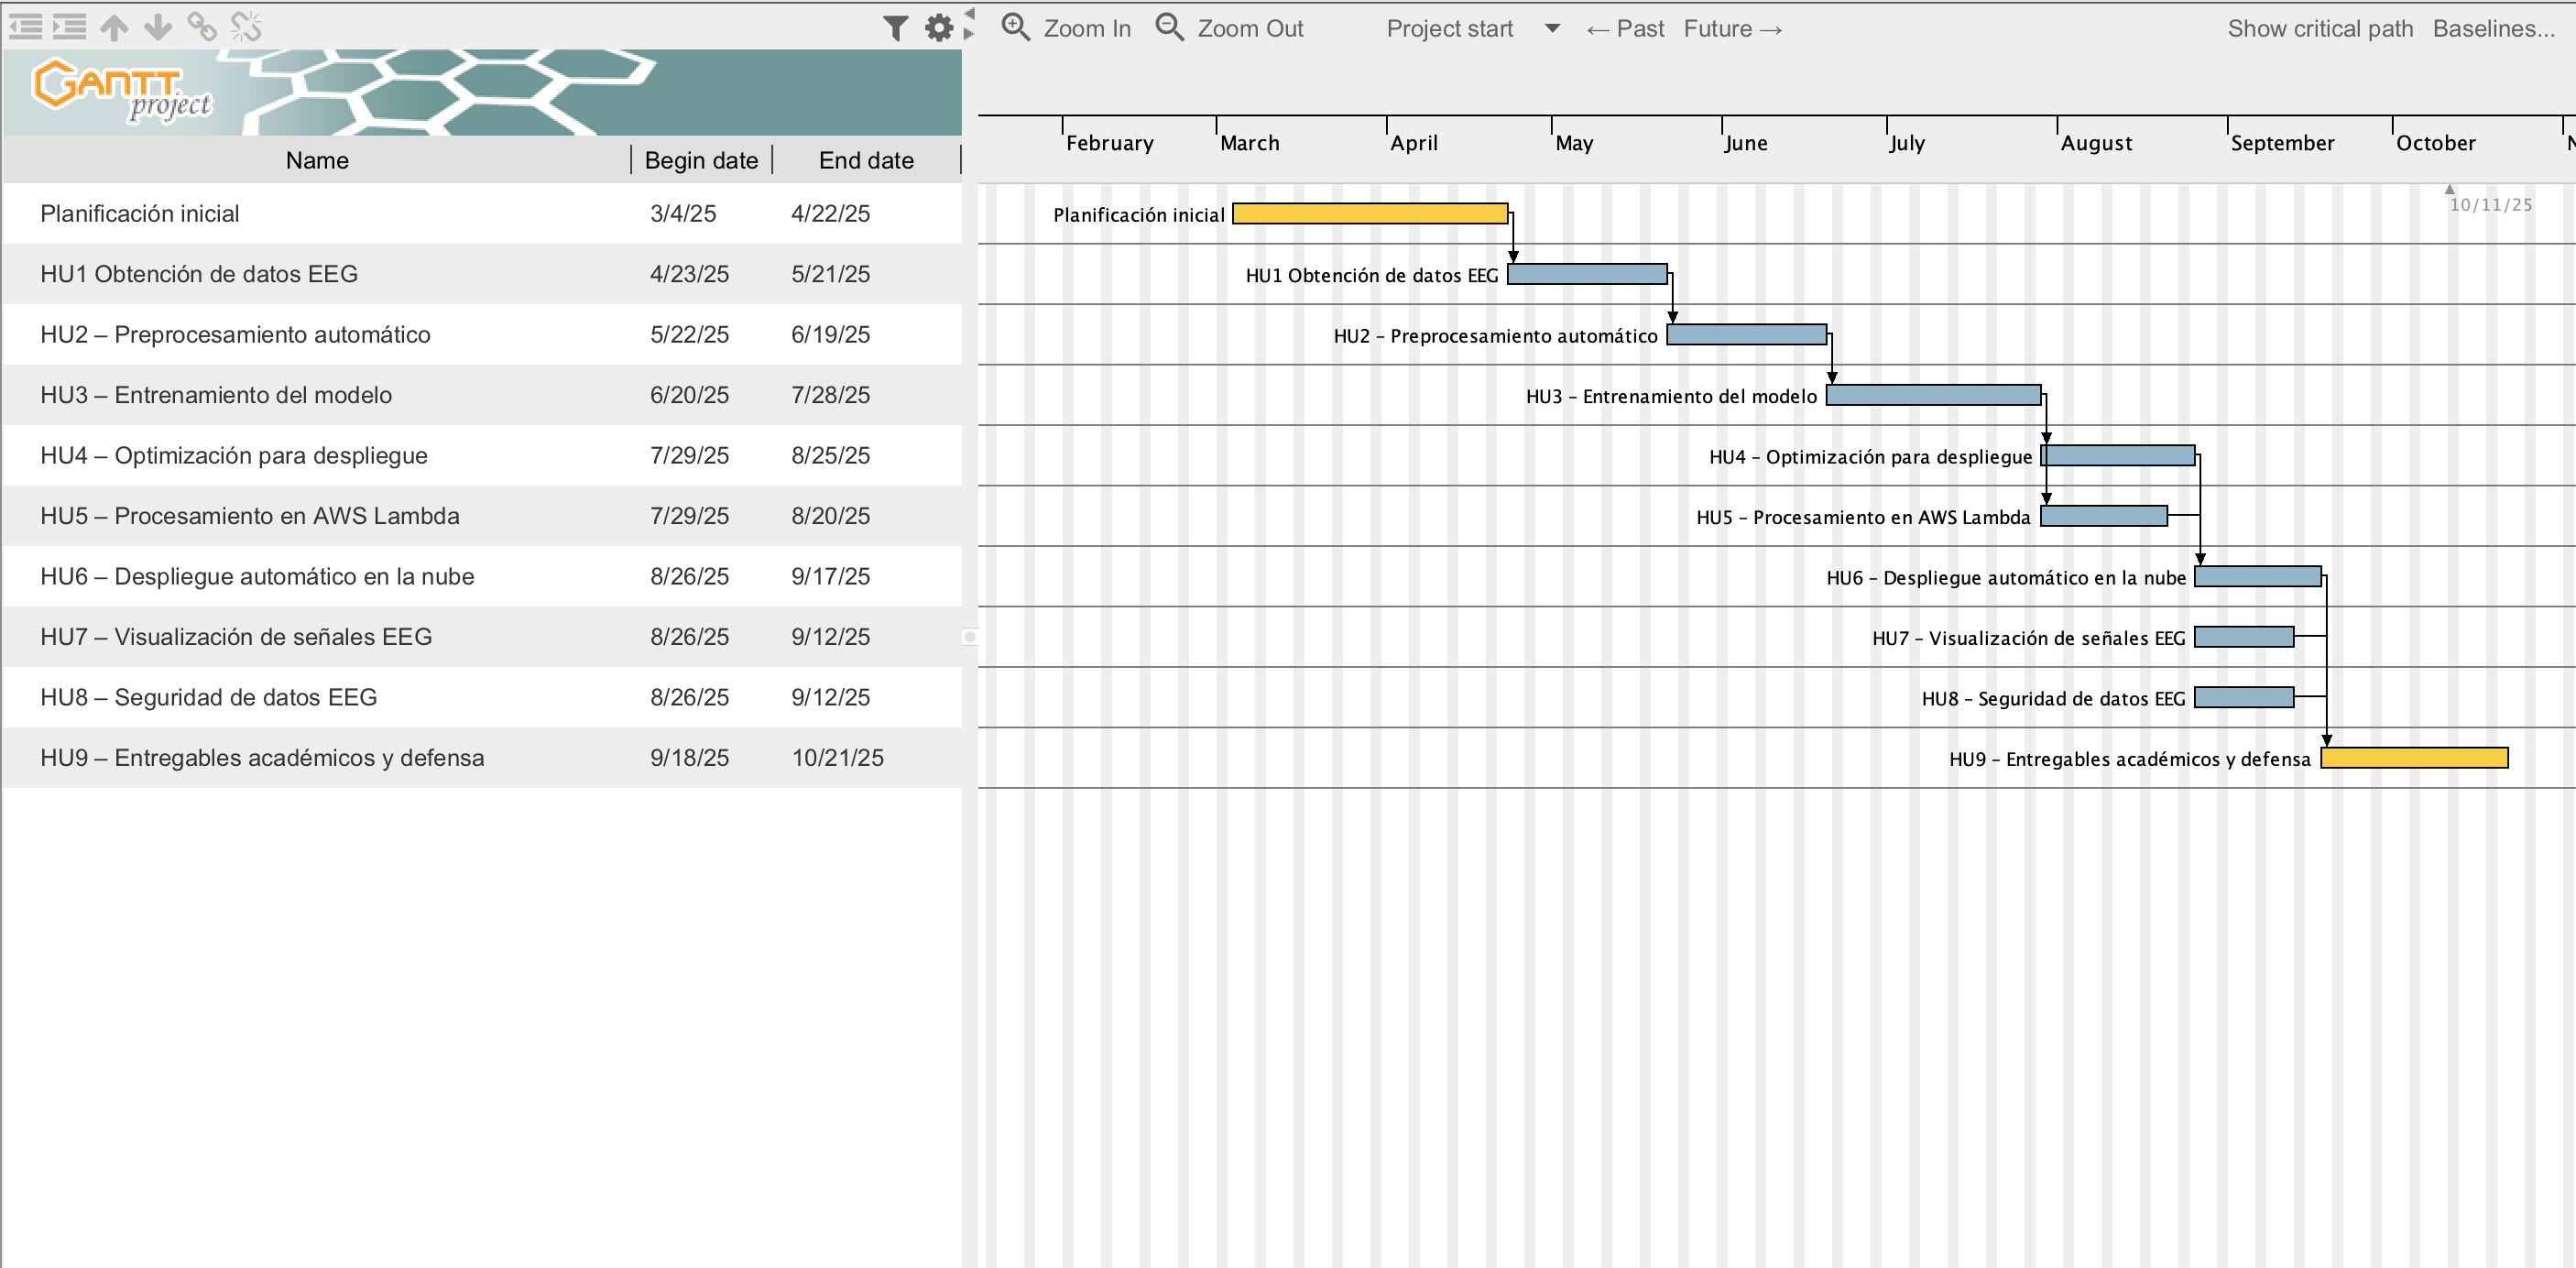
\includegraphics[width=.99\textwidth]{./Figuras/gant.png}
\caption{Diagrama de Gantt.}
\label{fig:diagBloques}
\end{figure}
\clearpage



\section{11. Planificación de Sprints}
A continuación, se detalla la tabla de planificación de Sprints.
\begin{table}[htpb]
\centering
\begin{tabularx}{\linewidth}{|l|>{\centering\arraybackslash}p{2.5cm}|X|>{\centering\arraybackslash}p{1.2cm}|>{\centering\arraybackslash}p{2.3cm}|>{\centering\arraybackslash}p{2.3cm}|}

% \begin{tabularx}{\linewidth}{@{}|l|l|X|c|l|c|@{}}
\hline
\rowcolor[HTML]{C0C0C0}
Sprint & HU & Tarea & Horas & Responsable & Completado \% \\ \hline
1 & HU1  & Exploración del dataset MOABB & 8 & Alumno & 0 \\ \hline
1 & HU1  & Análisis de estructuras de datos EEG & 8 & Alumno & 0 \\ \hline
1 & HU1  & Carga y limpieza de datos MOABB & 8 & Alumno & 0 \\ \hline
1 & HU1  & Documentación de la adquisición de datos & 8 & Alumno & 0 \\ \hline
2 & HU2  & Diseño del pipeline de preprocesamiento & 8 & Alumno & 0 \\ \hline
2 & HU2  & Implementación de filtrado y normalización & 8 & Alumno & 0 \\ \hline
2 & HU2  & Evaluación de calidad de señales preprocesadas & 8 & Alumno & 0 \\ \hline
2 & HU2  & Documentación de procesos y scripts & 8 & Alumno & 0 \\ \hline
2 & HU3  & Configuración de entorno virtual y dependencias & 4 & Alumno & 0 \\ \hline
2 & HU2  & Revisión de criterios de aceptación & 4 & Alumno & 0 \\ \hline
3 & HU3  & Definición de arquitectura del modelo & 8 & Alumno & 0 \\ \hline
3 & HU3  & Implementación y pruebas iniciales del modelo & 8 & Alumno & 0 \\ \hline
3 & HU3  & Validación cruzada y análisis de resultados & 8 & Alumno & 0 \\ \hline
3 & HU3  & Documentación del modelo & 8 & Alumno & 70 \\ \hline
4 & HU4  & Benchmarking con distintas configuraciones & 8 & Alumno & 0 \\ \hline
4 & HU4  & Optimización de tiempo de inferencia & 8 & Alumno & 0 \\ \hline
4 & HU4  & Pruebas de carga y latencia & 8 & Alumno & 0 \\ \hline
4 & HU4  & Exposición vía API REST & 8 & Alumno & 0 \\ \hline
5 & HU5  & Diseño arquitectura AWS (Lambda, API Gateway) & 8 & Alumno & 0 \\ \hline
5 & HU5  & Desarrollo funciones Lambda & 8 & Alumno & 0 \\ \hline
5 & HU5  & Pruebas de escalabilidad & 8 & Alumno & 0 \\ \hline
5 & HU5  & Seguridad básica y monitoreo & 8 & Alumno & 0 \\ \hline
\end{tabularx}
\end{table}


\begin{table}[htpb]
\centering
\begin{tabularx}{\linewidth}{|l|>{\centering\arraybackslash}p{2.5cm}|X|>{\centering\arraybackslash}p{1.2cm}|>{\centering\arraybackslash}p{2.3cm}|>{\centering\arraybackslash}p{2.3cm}|}
% \begin{tabularx}{\linewidth}{@{}|l|l|X|c|l|c|@{}}
\hline
\rowcolor[HTML]{C0C0C0}
Sprint & HU  & Tarea & Horas & Responsable & Completado \% \\ \hline
6 & HU6  & Configuración CI/CD para despliegue automático & 8 & Alumno & 0 \\ \hline
6 & HU6  & Integración con servicios de monitoreo & 8 & Alumno & 0 \\ \hline
6 & HU6  & Revisión de escalabilidad y rollback & 8 & Alumno & 0 \\ \hline
6 & HU6  & Pruebas y validación en entorno productivo & 8 & Alumno & 0 \\ \hline
7 & HU7  & Diseño de interfaz gráfica inicial & 8 & Alumno & 0 \\ \hline
7 & HU7  & Implementación de visualización de señales & 8 & Alumno & 0 \\ \hline
7 & HU7  & Exportación de datos a CSV y JSON & 8 & Alumno & 0 \\ \hline
7 & HU7  & Pruebas de usabilidad & 8 & Alumno & 0 \\ \hline
8 & HU8  & Implementación de cifrado en tránsito & 8 & Alumno & 0 \\ \hline
8 & HU8  & Implementación de cifrado en reposo & 8 & Alumno & 0 \\ \hline
8 & HU8  & Diseño de política de retención y eliminación & 8 & Alumno & 0 \\ \hline
8 & HU8  & Validación del cumplimiento de normativas & 8 & Alumno & 0 \\ \hline
9 & HU9 Planificación y memoria & Planificación inicial del proyecto & 8 & Alumno & 0 \\ \hline
9 & HU9 Planificación y memoria & Redacción del marco teórico & 8 & Alumno & 0 \\ \hline
9 & HU9 Planificación y memoria & Revisión bibliográfica & 8 & Alumno & 0 \\ \hline
9 & HU9 Planificación y memoria & Elaboración del índice de memoria & 8 & Alumno & 0 \\ \hline
10 & HU9 Planificación y memoria & Redacción de capítulos técnicos & 8 & Alumno & 0 \\ \hline
10 & HU9 Planificación y memoria & Integración de contenidos y estilo & 8 & Alumno & 0 \\ \hline
10 & HU9 Planificación y memoria & Revisión ortográfica y citación & 8 & Alumno & 0 \\ \hline
10 & HU9 Planificación y memoria & Creación de material para defensa & 8 & Alumno & 0 \\ \hline
\end{tabularx}
\end{table}


\begin{table}[htpb]
\centering
\begin{tabularx}{\linewidth}{|l|>{\centering\arraybackslash}p{2.5cm}|X|>{\centering\arraybackslash}p{1.2cm}|>{\centering\arraybackslash}p{2.3cm}|>{\centering\arraybackslash}p{2.3cm}|}
% \begin{tabularx}{\linewidth}{@{}|l|l|X|c|l|c|@{}}
\hline
\rowcolor[HTML]{C0C0C0}
Sprint & HU & Tarea & Horas & Responsable & Completado \% \\ \hline
11 & HU9 Finalización & Revisión global de entregables & 8 & Alumno & 0 \\ \hline
11 & HU9 Finalización & Simulacros de defensa & 8 & Alumno & 0 \\ \hline
11 & HU9 Finalización & Correcciones finales y ajustes & 8 & Alumno & 0 \\ \hline
11 & HU9 Finalización & Presentación ante jurado & 8 & Alumno & 0 \\ \hline
\end{tabularx}
\end{table}

\section{12. Normativa y cumplimiento de datos (gobernanza)}

En el presente proyecto, trabajará con datos de señales EEG provenientes de datasets públicos como MOABB (\textit{Mother of All BCI Benchmarks}), un repositorio público ampliamente utilizado en la comunidad científica para el estudio de interfaces cerebro-computadora. A continuación, se analizan los aspectos legales, éticos y técnicos relacionados con la gobernanza de estos datos.

\subsection*{12.1. Evaluación normativa aplicable}

Los datos EEG utilizados en este proyecto no contienen información de identificación personal (\textit{PII}), ya que han sido anonimizados previamente por las entidades que los generaron. No obstante, al tratarse de datos biométricos, pueden estar sujetos a regulaciones de privacidad según la jurisdicción. Se considera la siguiente normativa:

\begin{itemize}
  \item Reglamento General de Protección de Datos (GDPR - Unión Europea): establece que los datos biométricos se consideran datos sensibles y su tratamiento requiere garantías específicas, incluso si están anonimizados.
\end{itemize}

\subsection*{12.2. Consentimiento de los usuarios}

El dataset MOABB incluye únicamente registros cuya recolección fue realizada bajo protocolos éticos con consentimiento informado, documentado por las instituciones que lo generaron. Como usuario del dataset, el proyecto se adhiere a las licencias y restricciones de uso establecidas por los propietarios de los datos.

\subsection*{12.3. Restricciones de uso, compartición o publicación}

Los datos EEG empleados provienen de fuentes de acceso abierto, bajo licencias que permiten su uso para fines de investigación, con la condición de no intentar identificar a los sujetos participantes ni redistribuir los datos de forma desautorizada.

\subsection*{12.4. Fuente y licenciamiento de los datos}

Los datos utilizados pertenecen al proyecto MOABB \footnote{NeuroTechX, ``MOABB: Mother of All BCI Benchmarks,'' GitHub, disponible en: \url{https://github.com/NeuroTechX/moabb}} con licencia \textit{BSD 3-Clause License}
que ofrece múltiples datasets estandarizados para evaluación de modelos BCI. Se emplean únicamente los que están públicamente disponibles y cuentan con licencias de uso explícitas para investigación académica.

\subsection*{12.5. Consideraciones éticas y viabilidad legal}

Desde el punto de vista legal, el uso de MOABB como fuente de datos es viable para los fines del proyecto, siempre y cuando se respeten los términos de la licencia de uso y no se intente aplicar el sistema a datos personales sin consentimiento.

\subsection*{12.6. Gobernanza de los datos}

Se establece como principio del proyecto el cumplimiento del ciclo de vida de datos responsable, incluyendo:
\begin{itemize}
  \item Almacenamiento seguro y cifrado de los resultados.
  \item Eliminación periódica de datos temporales.
  \item Documentación clara sobre el uso y transformación de los datos.
  \item Evaluación de riesgos asociados a la exposición o mal uso de los datos.
\end{itemize}


\section{13. Gestión de riesgos}
\label{sec:riesgos}

Riesgo 1: retrasos en la adquisición o validación de datos
\begin{itemize}
    \item Severidad (S): 8 \\
    La falta de datos validados compromete el entrenamiento del modelo y la evaluación general del sistema.
    \item Ocurrencia (O): 5 \\
    Aunque los datos MOABB son de acceso abierto, la validación y el preprocesamiento pueden requerir más tiempo del esperado.
\end{itemize}

Riesgo 2: dificultad en el despliegue en AWS Lambda por límites técnicos
\begin{itemize}
    \item Severidad (S): 7 \\
    Superar límites de ejecución o memoria afectaría la escalabilidad del sistema.
    \item Ocurrencia (O): 6 \\
    La ejecución de modelos en tiempo real puede exceder los 15 segundos, especialmente en inferencia no optimizada.
\end{itemize}

Riesgo 3: falta de experiencia previa con MLOps y DevOps
\begin{itemize}
    \item Severidad (S): 6 \\
    El desconocimiento en herramientas que brindan automatización pueden retrasar la integración y despliegue continuo.
    
    \item Ocurrencia (O): 7 \\
    El desconocimiento del uso de las herramientas de automatización puede generar obstáculos técnicos, dado que el proyecto requiere el aprendizaje e implementación de estas herramientas, esto implica una curva de aprendizaje considerable.
\end{itemize}

Riesgo 4: vulnerabilidades en la seguridad de datos EEG
\begin{itemize}
    \item Severidad (S): 9 \\
    La filtración o uso indebido de datos EEG podría tener consecuencias legales y éticas graves.
    \item Ocurrencia (O): 4 \\
    Aunque se usan prácticas de cifrado, errores de configuración o descuidos pueden generar brechas.
\end{itemize}

Riesgo 5: sobrecarga de trabajo hacia el final del proyecto
\begin{itemize}
    \item Severidad (S): 6 \\
    Puede comprometer la calidad de entregables finales (documentación, defensa).
    \item Ocurrencia (O): 6 \\
    Hay alta probabilidad si no se sigue el cronograma de sprints rigurosamente.
\end{itemize}

\begin{table}[htpb]
\centering
\begin{tabularx}{\linewidth}{@{}|X|c|c|c|c|c|c|@{}}
\hline
\rowcolor[HTML]{C0C0C0}
\textbf{Riesgo} & \textbf{S} & \textbf{O} & \textbf{RPN} & \textbf{S*} & \textbf{O*} & \textbf{RPN*} \\ \hline
Retrasos en adquisición o validación de datos EEG & 8 & 5 & 40 & 6 & 3 & 18 \\ \hline
Dificultades técnicas en procesamiento en AWS Lambda & 7 & 6 & 42 & 6 & 4 & 24 \\ \hline
Inexperiencia en herramientas MLOps & 6 & 7 & 42 & 5 & 4 & 20 \\ \hline
Fallas en la seguridad de datos EEG & 9 & 4 & 36 & 6 & 3 & 18 \\ \hline
Sobrecarga de trabajo en etapas finales & 6 & 6 & 36 & 5 & 3 & 15 \\ \hline
\end{tabularx}


\end{table}
Criterio adoptado: se tomarán medidas de mitigación en los riesgos cuyos números de RPN sean mayores a \textbf{30}.

A continuación se presenta el plan de mitigación de los riesgos que exceden el RPN máximo establecido


Riesgo 1: retrasos en adquisición o validación de datos EEG
\begin{itemize}
  \item Plan de mitigación: asignar un sprint exclusivo para preprocesamiento y exploración de datasets. Revisión temprana de compatibilidad y calidad de datos.
  \item S* = 6: se reduce la severidad al distribuir la carga y revisar posibles fuentes alternativas.
  \item O* = 3: se reduce la ocurrencia al incorporar actividades preventivas y planificadas.
\end{itemize}

Riesgo 2: dificultades técnicas en AWS Lambda
\begin{itemize}
  \item Plan de mitigación: realizar pruebas de carga anticipadas con versiones reducidas del modelo. Optimizar uso de recursos desde etapas tempranas.
  \item S* = 6: se reduce al anticipar cambios arquitectónicos si son necesarios.
  \item O* = 4: disminuye gracias a pruebas en entorno de staging con métricas reales.
\end{itemize}

Riesgo 3: inexperiencia en herramientas MLOps
\begin{itemize}
  \item Plan de mitigación: planificación de capacitación autodidacta en los primeros sprints. Uso de plantillas y recursos oficiales de AWS.
  \item S* = 5: se reduce al adquirir familiaridad y estructurar procesos con ayuda.
  \item O* = 4:  baja gracias a tareas prácticas planificadas con revisión progresiva.
\end{itemize}

Riesgo 4: fallas en la seguridad de datos EEG
\begin{itemize}
  \item Plan de mitigación: Implementar cifrado en tránsito y en reposo desde el inicio. Aplicar políticas estrictas de permisos en los buckets y servicios involucrados.
  \item S* = 6: se reduce al incorporar prácticas estándar de ciberseguridad desde el diseño.
  \item O* = 3: baja gracias al uso de herramientas automatizadas de auditoría y monitoreo.
\end{itemize}

Riesgo 5: Sobrecarga de trabajo en etapas finales
\begin{itemize}
  \item Plan de mitigación: Distribuir la redacción de entregables en múltiples sprints y reservar buffers en el cronograma. Usar control de versiones también para la memoria escrita.
  \item S* = 5: baja al equilibrar mejor la carga desde etapas intermedias.
  \item O* = 3: disminuye al tener planificadas entregas parciales desde el sprint 6 en adelante.
\end{itemize}
\vspace{6.3cm}

\section{14. Sprint Review}
\label{sec:sprint_review}
\renewcommand{\arraystretch}{2.5}
\begin{table}[htpb]
\centering
\begin{tabular}{|>{\raggedright\arraybackslash}m{1.5cm}|
                >{\raggedright\arraybackslash}m{3cm}|
                >{\raggedright\arraybackslash}m{2.5cm}|
                >{\raggedright\arraybackslash}m{4cm}|
                >{\raggedright\arraybackslash}m{4cm}|}
\hline
\rowcolor[HTML]{CCCCCC}
\textbf{HU seleccionada} & \textbf{Tareas asociadas} & \textbf{Entregable esperado} & \textbf{¿Cómo sabrás que está cumplida?} & \textbf{Observaciones o riesgos} \\
\hline
                         & Exploración del dataset MOABB &                             &                                           &                                     \\ \cline{2-2}
\multirow{-2}{=}{HU1}    
                         & Limpieza y validación de señales EEG & 
\multirow{-2}{=}{Módulo funcional para adquisición de datos} & 
\multirow{-2}{=}{Cumple criterios de aceptación: datos limpios, cargados y validados} & 
\multirow{-2}{=}{Puede requerirse adaptar scripts para distintos formatos de dataset} \\
\hline
                         & Entrenamiento de modelo inicial &                             &                                           &                                     \\ \cline{2-2}
\multirow{-2}{=}{HU3}    
                         & Validación cruzada del modelo entrenado & 
\multirow{-2}{=}{Modelo entrenado y validado} & 
\multirow{-2}{=}{Métricas de desempeño alcanzadas con precisión mayor o igual a 80 \%} & 
\multirow{-2}{=}{Podrían surgir ajustes de hiperparámetros no previstos} \\
\hline
                         & Visualización de señales en interfaz gráfica &                             &                                           &                                     \\ \cline{2-2}
\multirow{-2}{=}{HU5}    
                         & Exportación de señales en CSV y JSON & 
\multirow{-2}{=}{Visualizador EEG funcional} & 
\multirow{-2}{=}{Gráficos legibles y exportaciones exitosas} & 
\multirow{-2}{=}{Riesgo en compatibilidad de formatos o librerías} \\
\hline
                         & Implementación de despliegue automático en AWS &                             &                                           &                                     \\ \cline{2-2}
\multirow{-2}{=}{HU6}    
                         & Configuración de monitoreo y pruebas & 
\multirow{-2}{=}{Modelo accesible vía API REST con CI/CD} & 
\multirow{-2}{=}{Endpoints activos y latencia medida en menor o igual a 15s} & 
\multirow{-2}{=}{Puede requerirse ajuste en recursos o permisos} \\
\hline
\end{tabular}
\end{table}





% \renewcommand{\arraystretch}{1.5}
% \begin{table}[H]
% \centering
% \begin{tabularx}{\linewidth}{|>{\raggedright\arraybackslash}p{3.2cm}|
%                                 >{\raggedright\arraybackslash}p{3.2cm}|
%                                 >{\raggedright\arraybackslash}X|
%                                 >{\raggedright\arraybackslash}p{3.2cm}|}
% \hline
% \rowcolor[HTML]{C0C0C0}
% \textbf{HU} & \textbf{Criterios de Aceptación} & \textbf{Método de Verificación} & \textbf{Observaciones Previstas} \\ \hline

% HU2 – Preprocesamiento EEG &
% Se deben aplicar filtros, normalizar señales y evaluar calidad. &
% Se ejecutarán scripts sobre datasets de prueba y se validará visual y estadísticamente la calidad de la señal. &
% Se prevé dificultad en señales con alto ruido o mala adquisición. \\ \hline

% HU3 – Entrenamiento de Modelo &
% El modelo debe ser entrenado correctamente y lograr métricas mínimas en validación. &
% Se comprobará mediante métricas (accuracy, F1-score) en conjunto de validación del pipeline. &
% Posible ajuste de hiperparámetros y reconsideración del modelo base. \\ \hline

% HU5 – Visualización EEG UI &
% La interfaz debe mostrar las señales y permitir exportar CSV y JSON. &
% Prueba funcional de la interfaz con simulaciones y test de exportación. &
% Se prevén ajustes menores en diseño o formatos de salida. \\ \hline

% HU6 – Despliegue en AWS &
% Modelo desplegado con monitoreo y escalabilidad básica configurada. &
% Verificación mediante logs, alertas y disponibilidad de endpoints de inferencia. &
% Dependencia de configuración en AWS; posible demora en permisos y acceso. \\ \hline

% \end{tabularx}
% \end{table}
% \vspace{0.5cm}

\section{15. Sprint Retrospective}    
\label{sec:sprint_retro}
\begin{table}[H]
\centering
\renewcommand{\arraystretch}{1.5}
\begin{tabularx}{\textwidth}{|>{\centering\arraybackslash}m{2.8cm}|
								  >{\raggedright\arraybackslash}X|
								  >{\raggedright\arraybackslash}X|
								  >{\raggedright\arraybackslash}X|
								  >{\raggedright\arraybackslash}X|
								  >{\raggedright\arraybackslash}X|}
\hline
\rowcolor[HTML]{C0C0C0}
\textbf{Sprint (tipo y N)} & \textbf{¿Qué hacer más?} & \textbf{¿Qué hacer menos?} & \textbf{¿Qué mantener?} & \textbf{¿Qué empezar a hacer?} & \textbf{¿Qué dejar de hacer?} \\
\hline
Sprint 0 (No técnico - Planificación ) &
Dedicar más tiempo a la planificación detallada y realista de tareas. &
subestimación de tiempos de documentación y revisión. &
La revisión cruzada de entregables antes de enviar. &
Hacer revisiones iterativas del cronograma a medida que avance el proyecto. &
Dejar de asumir que todas las tareas técnicas serán lineales en duración. \\
\hline
Sprint 2 (Técnico – Preprocesamiento EEG) &
Validar calidad de señal y documentación de \textit{scripts}. &
Optimizar código antes de validarlo. &
\textit{Pipeline} modular para reusabilidad y claridad. &
Usar validaciones automáticas en el flujo de preprocesamiento. &
Postergar tareas de documentación para el final. \\
\hline
Sprint 5 (Técnico – Extracción de características) &
Pruebas unitarias en etapas tempranas del desarrollo. &
Depender de notebooks desordenados. &
La automatización del \textit{pipeline} con \textit{scripts} parametrizables. &
Crear un repositorio limpio y separado para funciones reutilizables. &
Trabajar sin control de versiones fino por etapa. \\
\hline
Sprint 9 (Técnico – Entrenamiento y evaluación del modelo) &
Probar más métricas y evaluar resultados con mayor profundidad. &
Iteraciones sin documentación intermedia de resultados. &
La evaluación cruzada para robustez de resultados. &
Explorar herramientas para visualización de métricas. &
Almacenar resultados sólo localmente, sin respaldo en la nube. \\
\hline
\end{tabularx}
\end{table}
\end{document}